%%%%%%
%
% PROJECT 11 - Pest Control
%
% filename: pest_control.tex
% last modified: 2013-12-31
%
%%%%%%%
%
% IN THIS PROJECT, STUDENTS STUDY A SYSTEM OF TWO DIFFERENTIAL EQUATIONS THAT
% DESCRIBE THE INTERACTION BETWEEN MOSQUITOES AND DRAGONFLIES. PHASE PLANE ANALYSIS
% MAY BE USED HERE, ALTHOUGH I'M THINKING OTHER SOLUTION TECHNIQUES WILL WORK.
%
% COHEN, PAGE 463
%
%%%%%%%

\documentclass
[justified,nohyper]
{tufte-handout}

\usepackage{amsmath}

\usepackage{booktabs}
\usepackage{graphicx}
\usepackage{kmath,kerkis} % The order of the packages matters; kmath changes the default text font
\usepackage[T1]{fontenc}

\begin{document}
\section{Advanced Calculus Project 11: Pest Control}

\newthought{Predator-Prey models} use a system of two differential equations to study how two populations change over time. In class, we have looked at several of these kinds of models. In this project, our prey will be mosquitoes ($M$) and our predator will be dragonflies ($D$). The problem we need to solve is that the mosquito population sometimes is very high and sometimes is very low. We would like to better regulate the population of mosquitos.

Using the Lotka-Volterra model (fancy name for what we have already studied), we have the following system of two differential equations. $M$ and $D$ are functions of time and the constants $a$, $b$, $c$, and $d$ are related to how the two populations interact. For this project, $a$, $b$, $c$, and $d$ will remain fixed.

\begin{align*}
    M' &= aM - bMD \\
    D' &= -cD +dMD \\
\end{align*}

Using phase-plane analysis, we can plot the trajectories of the two populations. In the graph shown below, trajectories are represented by the colored curves that look like deformed circles. The arrows represent the slope field and have been colored to indicate growth speed. The best trajectories are the smallest, where the peaks of the mosquito population are not too large.

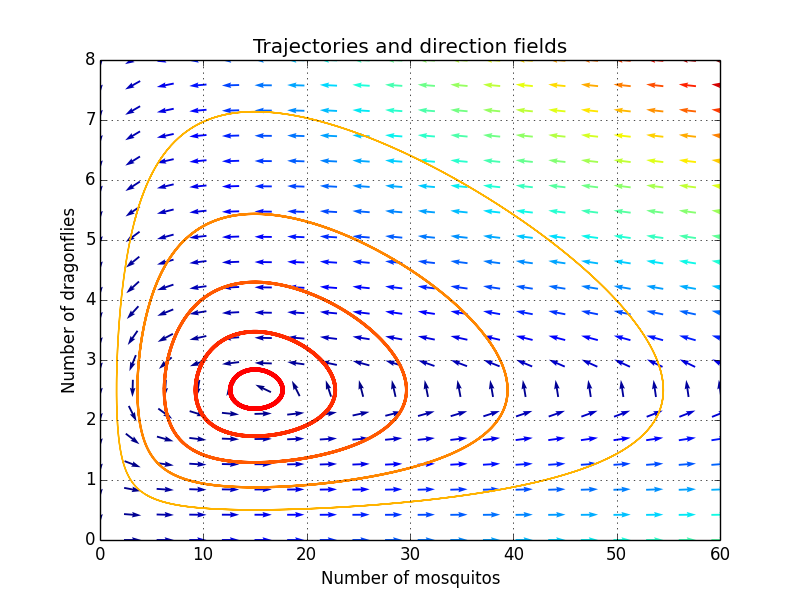
\includegraphics[scale=0.5]{field_mosquitos_and_dragonflies.png}

Suppose that we have a pesticide that kills mosquitos and not dragonflies. Using it, we reduce mosquitos, so we move to the left in the phase plane. The smart thing to do is to spray when the mosquito population is at its peak, because that would move us to a tighter curve.

Instead of high mosquito peaks and low valleys as shown below,

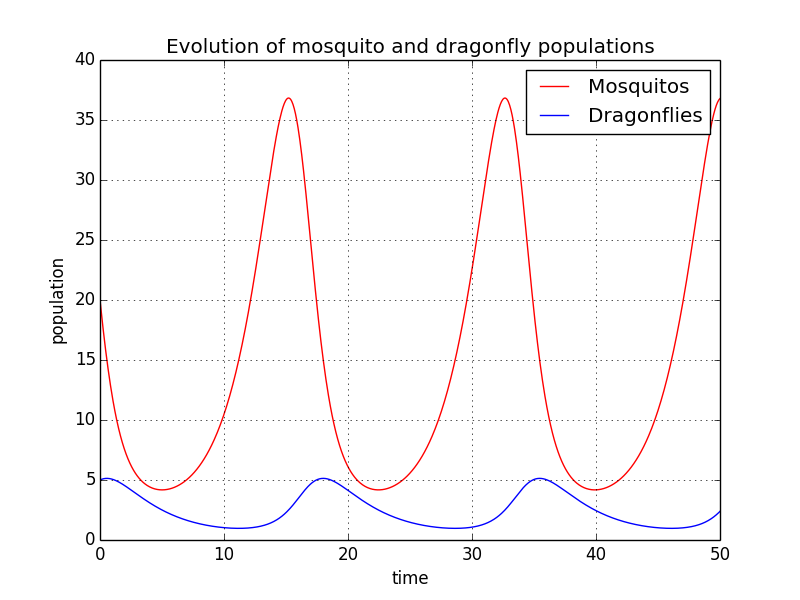
\includegraphics[scale=0.5]{pop_mosquitos_and_dragonflies_unregulated.png}

we'll have more moderate peaks and valleys. For example, if we kill mosquitos by spraying at time $t=15$, we can keep the population between 14 and 16.

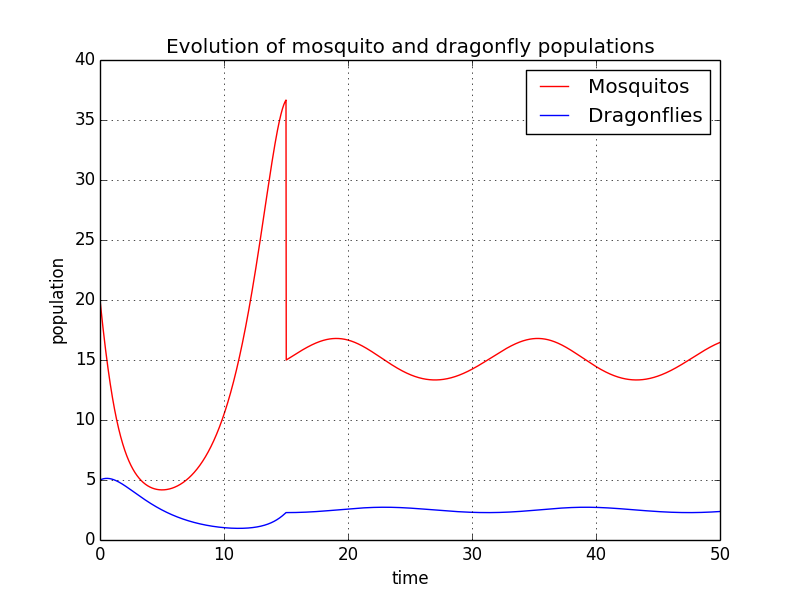
\includegraphics[scale=0.5]{pop_mosquitos_and_dragonflies_spray_at_peak.png}

But we have to be careful! If we spray at the wrong time, things could get worse. For example, if we spray when the mosquito population is at a minimum, this puts us on a larger trajectory and the mosquito population peaks are going to be higher than before we sprayed. In the graph shown below, the ``jump'' in mosquito population happens when we spray and instantaneously kill part of the mosquito population.

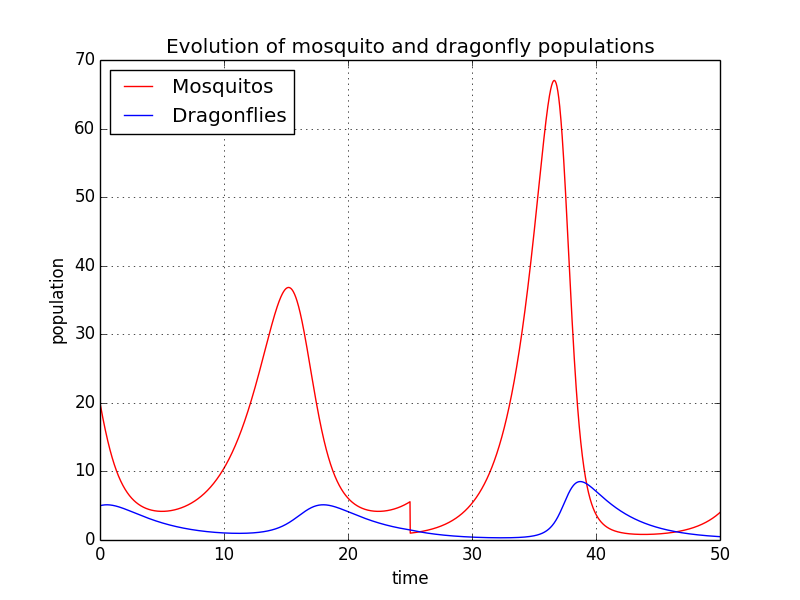
\includegraphics[scale=0.5]{pop_mosquitos_and_dragonflies_spray.png}

Imagine that you've been hired as a consultant to a small city which is considering spraying to control mosquitos. You've examined statistics on the mosquito population over the last 20 years and have constructed the following rough model of mosquito/dragonfly interaction:
\begin{align*}
    M' &= 0.5M - 0.2MD \\
    D' &= -0.3D + 0.1MD \\
\end{align*}
You estimate that currently $M=3$, $D=6$ (never mind what the units are). This point $(M,D)$ places us on one trajectory.

Prepare a concise written report suitable for presentation to the City Council. Address each of their five questions below. Keep your audience in mind, making your explanations and illustrations accessible to people who don't study the Calculus.

The City Council is considering five possible solutions to their mosquito problem. They will adopt the one you recommend, but they want to know your arguments for and against each one. Provide evidence in the form of diagrams, perhaps with some numerical information, to support your conclusions.

\begin{enumerate}
  \item Each dose of Pesticide \#1 kills half the mosquitos but doesn't affect the dragonflies. What would be the consequences of applying a dose when the mosquito population reaches its height? Should they use it more than once?
  \item Each dose of Pesticide \#2, which is cheaper, kills half of both populations. Is it worth trying? If so, at what point in the cycle should they apply it? Should they use it more than once?
  \item Would importing dragonflies help? If so, how many? (They are expensive.) And, more importantly, at what point in the cycle should they be released?
  \item One company offers to spray, on a regular basis, a chemical that cuts in half the reproductive rate of the mosquitos. Is this worth considering? (Hint: the reproductive rate determines a coefficient in the system of differential equations.)
  \item Finally, the firm that supplies dragonflies also has a different dragonfly that feeds on mosquitos. These would interbreed with the current dragonflies and change the equation for $D'$. Given equal numbers of mosquitos and dragonflies, the new mixed dragonfly population would be growing twice as fast. You'll also have to change the equation for $M'$ since the new population of dragonflies would eat mosquitos at half the current rate. Should the city buy the new dragonflies? Be sure to explain your recommendation.
\end{enumerate}


\end{document}